\documentclass[12pt, titlepage]{article}
\usepackage[a4paper,margin=.75in]{geometry}
\usepackage{tgtermes}
\usepackage{setspace}
\usepackage{placeins}
\usepackage{listings}
\usepackage{color}
\usepackage{fancyhdr}
\usepackage{graphicx}
\usepackage[parfill]{parskip}

\definecolor{dkgreen}{rgb}{0,0.6,0}
\definecolor{gray}{rgb}{0.5,0.5,0.5}
\definecolor{mauve}{rgb}{0.58,0,0.82}

\lstset{frame=none,
  language=Java,
  aboveskip=3mm,
  belowskip=3mm,
  showstringspaces=false,
  columns=flexible,
  basicstyle={\small\ttfamily},
  numbers=none,
  numberstyle=\tiny\color{gray},
  keywordstyle=\color{blue},
  commentstyle=\color{dkgreen},
  stringstyle=\color{mauve},
  breaklines=true,
  breakatwhitespace=true,
  tabsize=3
}

\pagestyle{fancyplain}
\lhead{Sean Connor}
\chead{Project 1 - Analysis}
\rhead{2 July 2018}

\title{Project 1 Analysis}
\author{Sean Connor \\ \\ 605.202 Data Structures \\ \\ 2 July 2018}
\date{}
\singlespacing

\begin{document}

\maketitle

\section {Data Structures}

In this project we were required to use the stack data structure, with a strict requirement being that language identification be accomplished via stack manipulation and counting in any way being forbidden. In addition, we were required to implement our own stack class, and not use Java's generic Stack$<$E$>$ class. While I believe that there are many ways to accomplish the goal of this project (language identification), using and manipulating a stack is a relatively simple solution.

First, a brief discussion of my implementation of the stack. I chose to use an array-based implementation due to its simplicity and ease of implementation and use. My implementation of stack is designed for use with the String data type, and will not work with any other type (i.e. char, int, etc). It includes a constructor which allows the user to initialize a String[] array of specified size which represents the stack. The size of the stack is fixed. If the number of characters in any line of the input file exceeds the hardcoded stack size (500), a stack overflow exception will be thrown. This is the main disadvantage of the array implementation of the stack.

Four essential methods are included - push(String item), pop(), peek(), and isEmpty(). With just these four methods one is able to accomplish the goal of the project. While it was revealed near the project deadline that comparing the number of items in the stack was acceptable, I included no methods to return the size of stack, as I was unsure if this would constitute counting. However, implementing this method is trivial.

With the Stack class in place, it was then a matter of employing stack manipulation to determine language.

\section{General Strategy}

The input was read line by line from a text file, with each line representing a different string to be evaluated. For each line, a number of methods included in my StringEval class are used to evaluate the string, and print the results to both the console and a new file using StringBuilder and BufferedWriter/OutputStreamWriter/FileOutputStream. These methods are aptly named type1, type2, type3, type4, and type5. 

The bulk of the project was found in designing algorithms that correctly identified languages using stacks and stack manipulation. The general strategy employed here was as follows:
\begin{enumerate}
	\item Test simple cases first (i.e. Is string empty? Is the first character an `A'?).
	\item Declare objects (i.e. Initialize the stack(s) to be used).
	\item Iterate through the string using a combination of a for-loop and the charAt(int location) methods.
	\item Perform language-specific stack manipulation.
	\item Exit loop. If stack is empty, return true. Else, return false.
\end{enumerate}
The language-specific stack manipulation varies substantially by language, and is best understood by viewing the source code. However, there was a common theme. When iterating through a string, if an `A' was encountered, push it to the stack. If a `B' was encountered, pop the stack. At the conclusion of the iteration, check if the stack was empty. If yes, return true.

One solution that I am particularly happy with was my solution to language 4. In this, I utilize two stacks and continually push/pop between the two. One stack is essentially used to store the order. The initial grouping establishes the order that must be maintained through the rest of the string, and is pushed to stack1. When popped to stack2, the top of stack2 is the same as the first item in the next grouping (if the string is a valid type 4). In this way, the order is continually checked as we iterate through the string.

\section{Algorithm Efficiency}

As described previously, the program first iterates through the input, line by line, and performs the language type evaluations on each string. Each language type evaluation method generally contains one or two non-nested for-loops that iterate through the characters in the string. Each stack function (push, pop, peek, isEmpty) features simple comparisons that are considered O(1). Considering this, I would expect the worst-case efficiency of the program to be O(n\textsuperscript{2}) due to the existence of nested for-loops. However, I am uncertain if this is the case, as the items which are being iterated through are different. In the nested for-loop, we iterate through the characters in the string, whereas in the parent for-loop we iterate through each line in the input file. The results would be quite different for 1000 lines of string length 5, 1000 lines of string length 1000, 5 lines of string length 1000, and 5 lines of string length 5.

To test this hypothesis (and provide enhancement to the program), I implemented a program execution timer and ran several test cases (n=5,50,100,500) with test cases beyond n=5 featuring repeats of the original five strings (average length = 5.4 and average length = 12). I then ran each test case five times and calculated the average time to execute. The results are presented in the figures below. Admittedly the sample size is small; however, we can see a linear trendline (R\textsuperscript{2} = 0.978 and R\textsuperscript{2} = 0.999). This is indicative of O(n) efficiency.

More testing would need to be done on this to get a better idea of performance at larger values of n and with longer string lengths. Perhaps in this case the numbers are simply too small to show the true nature of the efficiency of the algorithm. 

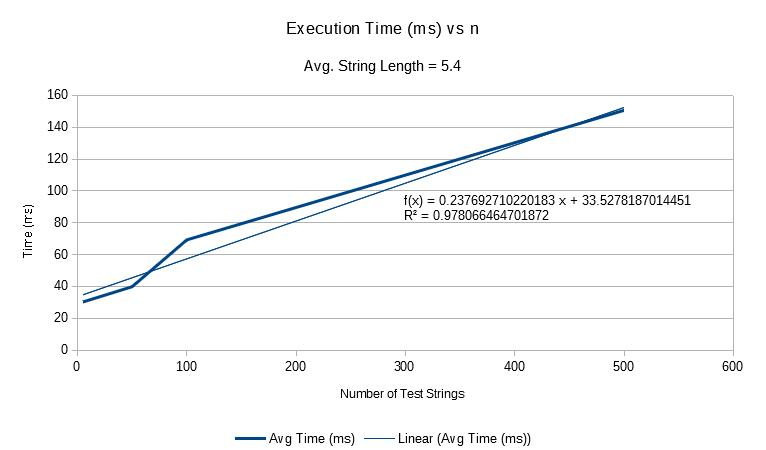
\includegraphics[width=\textwidth]{Efficiency}
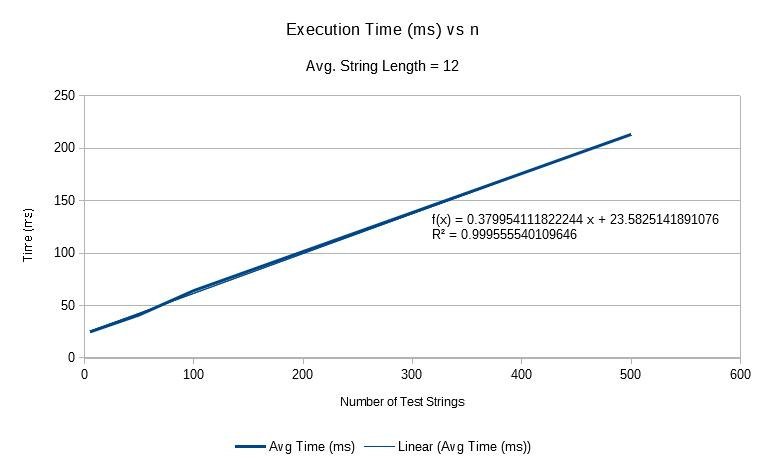
\includegraphics[width=\textwidth]{Efficiency2}

\section{Recursion}

Any iterative code can be converted to recursive and vice-versa. I'm still fairly new to recursion, so this was initially a bit tricky for me. However, with some thought, I realized it is simply a matter of implementing iteration in a recursive manner - that is, to call the same method but with a different parameter that ``increments" to the next step. 

I was not able to do this as simply a thought exercise - I had to create working recursive code as a proof of concept for at least one of the language evaluation methods. This code serves as an enhancement to the program, and is part of this document in the appendix (Section 6.1). Essentially, I include the same basic checks as the iterative method (in fact, I copy/pasted much of the code in the recursive method from the iterative method), but include an additional if-statement that invokes the recursive call until the last character of the string is reached. This same thought process can be applied to any of the other language evaluation methods - it is just a matter of making the iterative case `pseudo-iterative' using recursion.

Perhaps my recursive method is not very good, perhaps it could be optimized. But from initial inspection, I would argue that my iterative code is more efficient than my recursive code. My recursive code includes several statements that are redundant beyond the initial method call (such as checking if the string is empty or not). I would think that this reduces efficiency. If any iterative code can be replaced with recursive code and vice versa, then I think I will be sticking mostly with iterative methods, as it is simpler for me (at present time) to understand and implement. 

\section{Lessons Learned}

This was a great exercise in learning how to utilize the stack data structure. This is a great thing, because developing comfort in using a tool (data structure) expands the programmer's ``toolbox". This in turn expands the programmer's capabilities. I was most happy with my response to language type 4 for this very reason - I felt that I was really utilizing the stack/stack manipulation to accomplish the identification. 

In the same manner, thinking about this from a recursive view increases my comfort and capability in using and implementing recursion. So far, most of this class has been theory without much application. It felt great putting to practice the things we have been learning.

\newpage

\section{Appendix}
\subsection{Recursive Code for Language Type 1}
\begin{lstlisting}
/**
  * Recursive method to check for language type 1. This is functional code 
  * that correctly evaluates a string for language type 1.
  *
  * @param line   A string to be checked if posseses language type
  * @return   boolean value true if type 1, false otherwise
  */
private boolean type1rec(String line, Stack stack, String lc) {
        // check if string is empty
        // redundant recursively
        if (line.isEmpty()) {
            return true;
        }

        // check if there are any characters beside A and B in string
        // again, redundant recursively
        for (int i = 0; i < line.length(); i++) {
            lc = String.valueOf(line.charAt(i));

            if (!lc.equals("A") && !lc.equals("B")) {
                return false;
            }
        }

        // set lc to first char in string
        lc = String.valueOf(line.charAt(0));

        // push if stack empty or if same as top of stack
        // pop otherwise
        if (stack.isEmpty()) {
            stack.push(lc);
        } else {
            if (stack.peek().equals(lc)) {
                stack.push(lc);
            } else {
                stack.pop();
            }
        }

        // recursively iterate through string by using substring to `remove'
        // first character
        if (line.length() > 1) {
            line = line.substring(1,line.length());
            type1rec(line, stack, lc);
        }

        // at this point, all stack operations will have been performed after
        // iterating through entire string
        // redundant for all but first case
        if (stack.isEmpty()) {
            return true;
        } else {
            return false;
        }
}
\end{lstlisting}

\end{document}